\subsection{Inbetriebnahme}
\label{subsec:inbetriebnahme}

In diesem Kapitel wird die erste Inbetriebnahme des Roboters beschrieben.
Hierzu werden auch die Inhalte und Erweiterungen aufgelistet, welche im Lieferumfang für einen \gls{go1} Edu enthalten sind.
Anschließend soll der Betrieb durch den Akku und ein Netzteil beschrieben werden.

% todo an aus fernbedienung?
\subsubsection{Lieferumfang}

Abbildung \ref{fig:lieferumfang} zeigt die im Lieferumfang enthaltene Transportbox aus Styropor und deren Inhalte, welche
gleichzeitig der gesamte Lieferumfang des \gls{go1} in der \emph{Edu} Version ist.

\begin{figure}[h]
    \frame{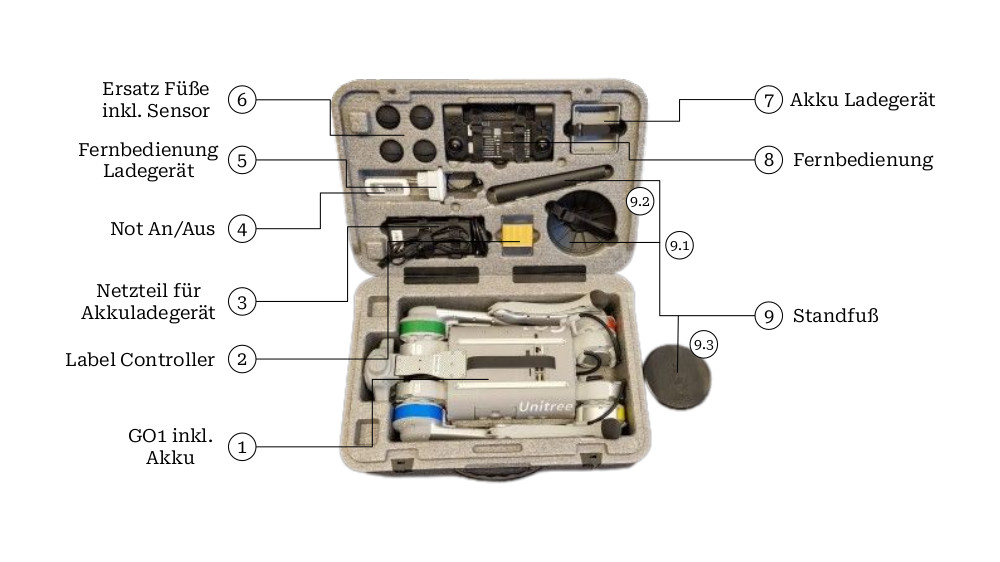
\includegraphics[width=\linewidth]{img/analyse/lieferumfang}}
    \caption{Ansicht der Transportbox und des Lieferumfangs}\label{fig:lieferumfang}
\end{figure}